% !TEX program = XeLaTeX
% !TEX encoding = UTF-8

\documentclass[a4paper]{article}

\usepackage[UTF8]{ctex}
\usepackage{graphicx}
\usepackage{soul, color, xcolor}
\usepackage[margin=1.25in]{geometry}
\usepackage{amsfonts, amsmath, amsthm, bm, amssymb}
\usepackage{float}
\usepackage{diagbox}
\usepackage{multirow}
\usepackage{hyperref}
\usepackage{listings}
\usepackage{tcolorbox}

\lstset{basicstyle=\tiny}

\setlength{\parindent}{0pt}

\numberwithin{equation}{section}

\theoremstyle{definition}
\newtheorem*{solution}{Solution}
\newtheorem*{prove}{Proof}

\def \transposed {\mathsf{T}}
\def \hermitian {\mathsf{H}}
\def \Real {\mathbb{R}}
\def \betaBold {\bm{\beta}}
\def \LambdaBold {\bm{\Lambda}}
\def \MuBold {\bm{\Mu}}
\def \muBold {\bm{\mu}}
\def \Sw {\mathbf{S}_{\mathrm{w}}}
\def \Sb {\mathbf{S}_{\mathrm{b}}}
\def \St {\mathbf{S}_{\mathrm{t}}}
\def \A {\mathbf{A}}
\def \B {\mathbf{B}}
\def \C {\mathbf{C}}
\def \O {\mathbf{O}}
\def \Q {\mathbf{Q}}
\def \I {\mathbf{I}}
\def \S {\mathbf{S}}
\def \M {\mathbf{M}}
\def \W {\mathbf{W}}
\def \X {\mathbf{X}}
\def \u {\bm{u}}
\def \v {\bm{v}}
\def \w {\bm{w}}
\def \wh {\hat{\bm{w}}}
\def \ws {\bm{w}^\star}
\def \y {\bm{y}}
\def \x {\bm{x}}
\def \xh {\hat{\bm{x}}}

% \let\oldnorm\norm
% \let\norm\undefined
\newcommand\abs[1]{\left| #1 \right|}
\newcommand\norm[1]{\left\| #1 \right\|}
\newcommand\inner[2]{\left\langle #1, #2 \right\rangle}
\newcommand\sbr[1]{\left( #1 \right)}
\newcommand\mbr[1]{\left[ #1 \right]}
\newcommand\lbr[1]{\left\{#1 \right\}}
\newcommand\tr[1]{\mathrm{tr}\sbr{#1}}
\newcommand\rank[1]{\mathrm{rank}\sbr{#1}}
\newcommand\indicator[1]{\mathbb{I}\sbr{#1}}

\begin{document}

\title{机器学习导论 习题二}
\author{221300066, 季千焜, \href{mailto:邮箱}{qkjiai@smail.nju.edu.cn}}
\maketitle

\section*{作业注意事项}

\begin{tcolorbox}
	\begin{enumerate}
		\item[1.] 作业所需的LaTeX及Python环境配置要求请参考: \href{https://www.lamda.nju.edu.cn/ML2024Spring/supplementary/environment.pdf}{[Link]};
		\item[2.] 请在LaTeX模板中第一页填写个人的学号、姓名、邮箱;
		\item[3.] 本次作业需提交的文件与对应的命名方式为:
		      \begin{enumerate}
			      \item [(a)] 作答后的LaTeX代码 --- \texttt{HW2.tex};
			      \item [(b)] 由(a)编译得到的PDF文件 --- \texttt{HW2.pdf};
			      \item [(c)] 编程题代码 --- \texttt{main.py};
		      \end{enumerate}
		      请将以上文件{\color{red}\textbf{打包为 ``\texttt{学号\hspace{0em}\_\hspace{0em}姓名.zip}''}}~(例如 ``\texttt{221300001\_\hspace{0em}张三.zip}'') 后提交;
		\item[3.] 若多次提交作业, 则在命名 ``\texttt{.zip}'' 文件时加上版本号, 例如 ``\texttt{221300001\_\hspace{0em}张三\hspace{0em}\_v1.zip}'' (批改时以版本号最高, 提交时间最新的文件为准);
		\item[4.] 本次作业提交截止时间为~{\color{red}\textbf{{4}月{19}日{23:59:59}}}. 未按照要求提交作业, 提交作业格式不正确, {\color{red}\textbf{作业命名不规范}}, 将会被扣除部分作业分数; 除特殊原因 (如因病缓交, 需出示医院假条) 逾期未交作业, 本次作业记 0 分; {\color{red}\textbf{如发现抄袭, 抄袭和被抄袭双方成绩全部取消}};
		\item[5.] 学习过程中, 允许参考 ChatGPT 等生成式语言模型的生成结果, 但必须在可信的信息源处核实信息的真实性; {\color{red}\textbf{不允许直接使用模型的生成结果作为作业的回答内容}}, 否则将视为作业非本人完成并取消成绩;
		\item[6.] 证明题请给出关键证明步骤, 计算题请列出算式及中间结果, 否则不予计分; 撰写数学表达式请遵循符号约定.
		\item[7.] 本次作业提交地址为 \href{https://box.nju.edu.cn/u/d/a84222be492048779a27/}{[Link]}, 请大家预留时间提前上交, 以防在临近截止日期时, 因网络等原因无法按时提交作业.
	\end{enumerate}
\end{tcolorbox}

\newpage

\section*{符号约定}

\textbf{[线性代数变量符号]} 本次作业的部分题目涉及矩阵形式的数学推导, 请注意符号规范.

提示: 可以在导言区通过 \texttt{\textbackslash{def}}, \texttt{\textbackslash{newcommand}} 等命令自定义常用符号以简化编写, 例如 \texttt{\textbackslash{Real}}, \texttt{\textbackslash{norm}} 等.

\begin{itemize}
	\setlength\itemsep{0em}
	\item 矩阵请使用\textbf{粗体正体字母}, 例如 $\A, \X, \O$ (零矩阵);
	\item 向量请使用\textbf{粗体斜体字母}, 例如 $\u, \v, \w, \x, \y, \bm{0}$ (零向量);
	\item 标量(以及离散变量)请使用\textbf{斜体小写字母}, 例如 $a, b, c, \lambda, \mu, \sigma$;
	\item 操作符或者函数名请使用\textbf{正体有衬线体字母}, 例如 $\min, \max, \mathrm{Ent}, \mathrm{MI}$;
	\item 转置矩阵 (Transposed Matrix) 以及埃尔米特矩阵 (Hermitian Matrix) 的\textbf{角标}请使用\textbf{正体无衬线体字母}, 例如 $\A^\transposed, \A^\hermitian$.
	% 注意: 请\textbf{不要}使用斜体字母 $T, H$, $\A^T, \A^H$ 将被视作矩阵之幂; 请\textbf{不要}使用 \texttt{\textbackslash{top}}, \texttt{\textbackslash{bot}}, $\top, \bot$ 常用于几何学, 逻辑学和抽象代数.
\end{itemize}

\textbf{[奇异值分解与特征值分解]} 由于 $\Real^n \times \Real^m$ 上存在全序关系, 我们可以约定, 存在一种奇异值分解过程, 在此奇异值分解过程的意义下, 任何矩阵的奇异值分解是唯一的, 进而\textbf{任何(半)正定矩阵的特征值分解也是唯一的}. 如果没有符号冲突, 可以不加说明的使用以下记号:

\begin{itemize}
	\setlength\itemsep{0em}
	\item 矩阵 $\A \in \Real^{n \times m}$ 的\textbf{奇异值分解}是 $\A = \sum_{i=1}^{\min\{m,n\}} \sigma_i \u_i \v_i^\transposed$, $\sigma_i \geqslant \sigma_{i+1}$;
	\item \textbf{(半)正定} 矩阵 $\A \in \Real^{n \times n}$ 的\textbf{特征值分解}是 $\A = \sum_{i=1}^{n} \lambda_i \v_i \v_i^\transposed$, $\lambda_i \geqslant \lambda_{i+1}$;
	\item 另记 $\sigma_{\max}(\A) = \sigma_1(\A), \lambda_{\max}(\A) = \lambda_1(\A)$ 是矩阵 $\A$ 最大的奇异值.
\end{itemize}

\textbf{[决策树]} 为简化表述, 我们引入指示函数 $\indicator{e}$: 若事件 $e$ 发生, 则 $\indicator{e} = 1$, 否则 $\indicator{e} = 0$. 对于\textbf{表格数据}, 我们约定:

\begin{itemize}
	\setlength\itemsep{0em}
	\item 每个样例 $\x$ 都具有 $d$ 个属性 $\{1, \cdots, d\}$;
	\item 第 $j$ 个属性有 $n_j$ 种可能的取值, 记作 $\x^j \in \{v^j_1, \cdots, v^j_{n_j}\}$;
	\item 对于多分类问题, 样例的标签可以记作 $\x^\ell$, 共有 $N$ 种可能取值, 即 $\x^\ell \in \{1, \cdots, N\}$.
\end{itemize}

例如: 对于数据集 $D = \{\x_1, \cdots, \x_m\}$, 事件 $\x^j = v^j_k$ 的频率值可以记作 $\hat{p}(\x^j = v^j_k) = \frac{1}{m} \sum_{i=1}^{m} \indicator{\x_i^j = v^j_k}$; 再如, 对于 ``西瓜数据集2.0'' (详见教材表4.1), 记号示范如下:

\begin{itemize}
	\setlength\itemsep{0em}
	\item $d = 6$;
	\item $\x^1 \in \{v^1_1=\text{乌黑}, v^1_2=\text{青绿}, v^1_3=\text{浅白}\}$, 即第1个属性色泽, $n_1 = 3$;
	\item $\x^2 \in \{v^2_1=\text{蜡缩}, v^2_2=\text{稍蜷}, v^2_3=\text{硬挺}\}$, 即第2个属性根蒂, $n_2 = 3$;
	\item $\x^3 \in \{v^3_1=\text{清脆}, v^3_2=\text{浊响}, v^3_3=\text{沉闷}\}$, 即第3个属性敲声, $n_3 = 3$;
	\item $\x^4 \in \{v^4_1=\text{清晰}, v^4_2=\text{稍糊}, v^4_3=\text{模糊}\}$, 即第4个属性纹理, $n_4 = 3$;
	\item $\x^5 \in \{v^5_1=\text{凹陷}, v^5_2=\text{稍凹}, v^5_3=\text{平坦}\}$, 即第5个属性脐部, $n_5 = 3$;
	\item $\x^6 \in \{v^6_1=\text{软粘}, v^6_2=\text{硬滑}\}$, 即第6个属性触感, $n_6 = 2$.
\end{itemize}

\newpage

\section{[20pts] 岭回归}

在本题中, 我们假设\textbf{所有凸优化问题均有解}.

回顾教材第三章第二节, 多元线性回归相当于求解如下的无约束优化问题 \eqref{lr}. 其中, 对于 $\v \in \Real^d$, 定义 $\norm{\v}_2^2 = \v^\transposed \v$.
\begin{equation}
	\min_{\wh} \quad\norm{\X\wh - \y}_2^2
	\label{lr}
\end{equation}
在多元线性回归中增加约束项, 即成为\textbf{岭回归 (Rigde Regression}), 即求解有约束优化问题 \eqref{ridge-rho}, 其中 $\rho > 0$ 是待确定的超参数.
\begin{equation}
	\begin{aligned}
		\min_{\wh} \quad  & \norm{\X\wh - \y}_2^2           \\
		\text{s.t.} \quad & \norm{\wh}_2^2 \leqslant \rho^2 \\
	\end{aligned}
	\label{ridge-rho}
\end{equation}
岭回归也可以写成无约束优化问题 \eqref{ridge-lambda}. 其中, $\lambda \geq 0$ 是待确定的超参数.
\begin{equation}
	\begin{aligned}
		\min_{\wh} \quad\norm{\X\wh - \y}_2^2 + \lambda \norm{\wh}_2^2
	\end{aligned}
	\label{ridge-lambda}
\end{equation}

\begin{itemize}
	\item[(1)] \textbf{[5pts]} 相比于多元线性回归, 岭回归引入了额外的\textbf{归纳偏好 (Inductive Bias)}. 回顾教材第一章第四节, 请简要回答: 岭回归引入了怎样的归纳偏好? 这样的归纳偏好有怎样的作用? \\
	      提示: 回顾\textbf{过拟合 (Overfitting)、``奥卡姆剃刀'' (Occam's Razor) 原则}等知识点; 结合特殊情形回答, 例如矩阵 $\X$ 不满秩、数据中存在异常值等.
	\item[(2)] \textbf{[5pts]} 请证明岭回归的两种形式 \eqref{ridge-rho} 和 \eqref{ridge-lambda} 等价. \\
	      提示:考虑 \textbf{KKT条件 (Karush-Kuhn-Tucker Conditions)}.
	\item[(3)] \textbf{[5pts]} 对于无约束优化形式 \eqref{ridge-lambda}, 假设 $\lambda$ 已经确定, 此时岭回归的解记作 $\ws$, 请推导出 $\ws$ 的表达式.
	\item[(4)] \textbf{[5pts]} \textbf{在 (3) 的基础上}, 请推导出 $\lambda$ 的下界 (关于 $\rho$ 的函数), 并据此回答: $\rho$ 减小时, 若希望保持 \eqref{ridge-rho} 和 \eqref{ridge-lambda} 的解一致, 需要怎样调整 $\lambda$? \\
	      提示: 你可能需要引入 $\sigma_{\max}(\X)$.
\end{itemize}

\begin{solution}
此处用于写解答 (中英文均可)\\
(1)归纳偏好:岭回归希望让解向量 $\hat{\w}$ 在满足能够最小化 $\|\X\hat{\w} - \y\|_{2}^{2}$ 的同时,更加偏好于那些在欧几里得空间中的模长尽量小,不超过一个超参数 $\rho$ 的解向量。
\\
作用:\\
1. 首先最小化 $\|\X\hat{\w} - \y\|_{2}^{2}$ 是一个无约束的优化问题,那么可转化为求解能够使 $2\X^{T}(\X\w^{*}-\y) = \textbf{0\textbf{}}$ 的 $\hat{\w}$。那么如果 $\X^{T}\X$ 满秩的话,有唯一的闭式解;如果不满秩的话,那么满足这个式的 $\hat{\w}$ 会构成一个解空间。引入这个归纳偏好后,岭回归算法会挑选 $2$ 范数不超过超参数 $\rho$ 的解(根据奥卡姆剃刀原则,某种程度上可以认为这种解的形式更加简单)。\\
2. 原始的线性回归是通过最小化均方误差来得到解,而均方误差对异常值很敏感,容易导致出现对某一项指标的过分偏重。而岭回归通过引入一个正则化项去惩罚过大的 $\hat{\w}$,从而减小了异常值对于最优解的影响,以在存在较大噪声的前提下达到更好回归的效果。\\
(2)证明:

(1.2) 式中的$\|\X\hat{\w} - \y\|^2$ 显然是关于 $\hat{\w}$ 的凸函数,同理因为 $\lambda \geq 0$,(1.3) 式中的 $\|\X\hat{\w} - \y\|^2 + \lambda\|\hat{\w}\|^2$ 也是关于 $\hat{\w}$ 的一个凸函数。
由式 (1.3) 是凸函数,可立即得到其最优解满足下面的式子:
$$
\frac{\partial\|\X\hat{\w} - \y\|^2 + \lambda\|\hat{\w}\|^2}{\partial \w} = 2\X^T(\X\hat{\w} - \y) + 2\lambda \w = \textbf{0}
$$
通过整理可得最优解 $\hat{\w}$ 满足下式:
$$(\X^T\X+\lambda\I)\hat{\w}=\X^T\y$$
由式 (1.2) 以及其约束条件可知,这是一个凸优化问题,所以满足 KKT 条件的点就是其最优解,其 KKT 条件如下:
$$
\| \hat{\w} \|_{2}^{2} - \rho^2 \leq 0 $$
$$ 
\mu \geq 0$$
$$
\mu(\|\hat{\w}\|_{2}^{2} - \rho^2) = 0 $$ 
$$
2\X^T(\X\hat{\w} - \y) + 2\mu \hat{\w} = \textbf{0}
$$
那么要证明这两个优化问题等价,即证明:
$$1.\forall\lambda \geq 0,\exists\rho > 0,s.t.\hat{\w_{1}} = \hat{\w_{2}}$$
$$2.\forall\rho > 0,\exists\lambda \geq 0,s.t.\hat{\w_{2}} = \hat{\w_{1}}
$$
下面规定: $\hat{\w_{1}}, \hat{\w_{2}}$ 分别是 (1.2),(1.3) 取得最优解时 $\hat{\w}$ 的值。\\
证明1:\\
对 $\forall\lambda > 0$,因为有对于任意 $\hat{\w}$,$\hat{\w}^T \X^T \X\hat{\w} = (\hat{\w}\X)^T (\hat{\w}\X) \geq 0$,则 $\X^T\X$ 一定是半正定矩阵,所以 $\X^T \X + \lambda \I$ 一定是正定矩阵,所以它可逆,$\hat{\w_{2}}$ 有唯一解,所以有 $\hat{\w_{2}} = (\X^T \X + \lambda \I)^{-1}\X^T \y$。\\
此时来观察 KKT 条件,只需令 $\mu = \lambda$,$\rho = \|(\X^T\X + \lambda \I)^{-1}\X^T \y\|$,取 $\hat{\w_{1}}= \hat{\w_{2}}$即可满足 KKT 条件,所以有 $\hat{\w_{1}}= \hat{\w_{2}}$ 是 $\rho = \|(\X^T\X + \lambda \I)^{-1}\X^T \y\|$ 的条件下问题 (1.2) 的解。\\
当 $\lambda = 0$ 时,令 $\mu = 0$,因为 $\X^T\X$ 半正定,所以解出来的 $\hat{\w_{2}}$ 的集合是一个子空间,对于该解空间中任意的 $\hat{\w_{2}}$,只需令 $\rho = \|\hat{\w_{2}}\|$即可满足 KKT 条件,即可以得到 $\hat{\w_{1}}= \hat{\w_{2}}$.\\
证明2:\\
对 $\forall\rho > 0$,取 KKT 条件中 $\|\hat{\w} _{2}^{2}\| = \rho^2$,必须让 $\hat{\w_{1}}$满足 $2\X^T (\X\hat{\w_{1}} - \y) + 2\mu \hat{\w_{1}} = \textbf{0}$,且此时 $\mu$依赖于 $\rho$的值。根据之前的分析可以解得 $\hat{\w_{1}} = (\X^T \X + \mu \I)^{-1}\X^T \y$, 因为此时 $\|\hat{\w_{1}}\| = \rho^2$,取能够满足 $(\X^T\X + \mu \I)^{-1}\X^T\y^2 = \rho^2$的大于 $0$的 $\mu$即可,此时再令 $\lambda = \mu$,即可得到 $\hat{\w_{2}}= \hat{\w_{1}}$.\\
下面讨论一种特殊情况,即找不到 $\mu > 0$满足 $\|(\X^T \X + \mu \I)^{-1} \X^T\y \| = \rho^2$,因为变大 $\mu$实际上是在缩小 $\X^T\y$的模长,所以出现这种情况说明 $\rho$的值很大,那么就取不到 $\|\hat{\w_{1}}\|_{2}^{2} = \rho^2$,因而此时有 $\|\hat{\w_{1}}\|_{2}^{2} < \rho^2$,令 $\mu = 0$,$\lambda = 0$,就可以找到 $\hat{\w_{2}}= \hat{\w_{1}}$.\\
综上,可以证明这两个条件是等价的。\\
(3)通过 $(2)$中的推导,易得:\\
当 $\lambda > 0$时:
$$
\ws=(\X^T\X+\lambda\I)^{-1}\X^T\y$$
当 $\lambda = 0$时:
$$
\ws=(\X^T\X)^{-1}\X^T\y
$$
(4)$\lambda$应该调大。\\
从(2)的分析中可以得到,当这两个问题等价时,有:
$$
\rho \geq \|(\X^T\X + \lambda \I)^{-1}\X^T\y\|_{2}$$
因为 $\X^T\y$得到的是一个向量,又因为 $\X^T\X$是半正定矩阵,选取其最大特征值 $\sigma_{\text{max}}(\X^T\X)$,根据高等代数的相关结论,有 $(\X^T\X + \lambda \I)^{-1}$的最小特征值为 $\frac{1}{\lambda+\sigma_{\text{max}}(\X^T\X)}$,那么显然有:$$
\rho \geq \|(\X^T\X+\lambda \I)^{-1}\X^T\y\|_{2}\geq \frac{\|\X^T\y\|_{2}}{\lambda+\sigma_{\text{max}}(\X^T\X)} $$
在这里第二个不等号能够成立是因为 $(\X^T\X + \lambda \I)^{-1}$相当于对向量做了正交变换后伸缩其基的长度,那么当该向量与被缩短最明显的向量平行时,其模长最小.不难得到 $\lambda$的下界为:$$
\lambda \geq \frac{\|\X^T\y\|_{2}}{\rho}-\sigma_{\text{max}}(\X^T\X)
$$
显然 $\lambda$的下界是关于 $\rho$的减函数,所以当 $\rho$减小时,$\lambda$的下界会变大,此时应该将 $\lambda$相应地调大。
\end{solution}

\newpage

\section{[20pts] 决策树的构建流程}

\begin{tcolorbox}
	\textbf{[注意事项]} 本题可使用 PowerPoint\textsuperscript{\textregistered}, Visio\textsuperscript{\textregistered} 等软件软件绘制决策树, 导出为图片或 PDF 插入到作业文档中; 亦允许手绘决策树, 但是请确保文字与线条的工整. 如果插入照片, 请确保照片内容清晰可读, 否则将扣除部分分数.
\end{tcolorbox}

考虑如下的表格数据集: 在诊断疾病 RD 时, 通常采用 UW-OCT, OCT-PD, US 三种检测手段, 其中 1 代表阳性, 0 代表阴性. 假设总共收集了 16 位病人的检测结果, 其中 8 条用于训练, 如表格 \ref{dt-train} 所示, 8 条用于验证, 如表格 \ref{dt-valid} 所示.

\begin{table}[ht]
	\centering
	\setlength{\abovecaptionskip}{0pt}
	\setlength{\belowcaptionskip}{5pt}
	\caption{训练集 $D_{\mathrm{train}}$}
	\label{dt-train}
	\begin{tabular}{cccc|c}
		\hline
		编号 & UW-OCT & OCT-PD & US & RD \\
		\hline
		1  & 1      & 1      & 0  & 1  \\
		2  & 1      & 1      & 1  & 1  \\
		3  & 0      & 1      & 1  & 1  \\
		4  & 0      & 1      & 1  & 1  \\
		5  & 0      & 0      & 1  & 0  \\
		6  & 1      & 0      & 0  & 0  \\
		7  & 1      & 0      & 1  & 0  \\
		8  & 0      & 1      & 0  & 0  \\
		\hline
	\end{tabular}
\end{table}

\begin{table}[ht]
	\centering
	\setlength{\abovecaptionskip}{0pt}
	\setlength{\belowcaptionskip}{5pt}
	\caption{验证集 $D_{\mathrm{valid}}$}
	\label{dt-valid}
	\begin{tabular}{cccc|c}
		\hline
		编号 & UW-OCT & OCT-PD & US & RD \\
		\hline
		9  & 1      & 1      & 1  & 1  \\
		10 & 0      & 1      & 1  & 1  \\
		11 & 0      & 1      & 0  & 0  \\
		12 & 1      & 0      & 1  & 0  \\
		13 & 0      & 1      & 1  & 1  \\
		14 & 1      & 1      & 0  & 0  \\
		15 & 1      & 0      & 0  & 0  \\
		16 & 0      & 0      & 0  & 0  \\
		\hline
	\end{tabular}
\end{table}

\begin{enumerate}
	\item[(1)] \textbf{[10pts]} 回顾教材第四章第一, 二节, 请使用基尼指数作为划分准则, 通过训练集中的数据训练决策树. 在 \texttt{HW2.pdf} 中展示\textbf{最终得到的决策树}, 并给出\textbf{每个节点划分时的计算和比较过程}.
	\item[(2)] \textbf{[5pts]} 回顾教材第四章第三节, 在(1)的基础上, 请判断每个节点是否需要预剪枝. 在 \texttt{HW2.pdf} 中展示\textbf{预剪枝后的决策树}, 并给出\textbf{每个节点预剪枝时的计算和比较过程}.
	\item[(3)] \textbf{[5pts]} 对一个学习任务来说, 给定属性集, 其中有些属性可能很关键, 很有用, 称为 ``相关特征'', 另一些属性则可能用处不大, 称为 ``无关特征''. 请简要回答如下问题:
	      \begin{itemize}
		      \item[(a)] 比较 (1,2) 的结果, 指出当前训练集和验证集划分下的无关特征, 并说明理由.
		      \item[(b)] 如果不给出数据集, 只给出决策树和剪枝后的决策树, 应该怎样挑选无关特征?
		      \item[(c)] 如果不给出数据集, 也不给出剪枝后的决策树, 只给出未剪枝的决策树, 还能挑选无关特征吗? 请简要给出理由.
	      \end{itemize}
\end{enumerate}

\begin{solution}
	此处用于写解答 (中英文均可)\\
 (1)在还是根结点时,当前属性集合为$\lbrace UW-OCT, OCT-P D, US\rbrace$,对每个属性,都有 $\lbrace 0, 1 \rbrace$ 两个取值,所以对于所有属性的基尼值:

$Gini(D, UW-OCT = 1) = 1 − (1/2)^2 − (1/2)^2 = 1/2$

$Gini(D, UW-OCT = 0) = 1 − (1/2)^2 − (1/2)^2 = 1/2$

$Gini(D, OCT-PD = 1) = 1 − (4/5)^2 − (1/5)^2 = 8/25$

$Gini(D, OCT-PD = 0) = 1 − (0 + 1) = 0$

$Gini(D, US = 1) = 1 − (3/5)^2 − (2/5)^2 = 12/25$

$Gini(D, US = 0) = 1 − (1/3)^2 − (2/3)^2 = 4/9$

可以求得各属性的基尼系数为:

$Gini\_index(D, UW-OCT) = 4/8 × 1/2 + 4/8 × 1/2 = 1/2$

$Gini\_index(D, OCT-P D) = 5/8 × 8/25 + 3/8 × 0 = 1/5$

$Gini\_index(D, US) = 5/8 × 12/25 + 3/8 × 4/9 = 7/15$

因为 OCT-PD 的基尼系数最小,可以设置为划分属性,得到以下决策树:
 \begin{figure}[H]
    \centering
    \includegraphics[width=0.8\textwidth]{决策树构建流程1.png}\\
    \caption{决策树构建流程1}
    \label{fig:roc}
\end{figure}

可以发现右子树中样例都是阴性,可直接设为阴性。接下来,我们计算左边集合各个属性的基尼值:

$Gini(D1, UW-OCT = 1) = 1 − (1 + 0) = 0$

$Gini(D1, UW-OCT = 0) = 1 − \frac{2}{3} × \frac{2}{3} = \frac{4}{9}$

$Gini(D1, US = 0) = 1 − (1 + 0) = 0$

$Gini(D1, US = 1) = 1 − \frac{1}{2} × \frac{1}{2} = \frac{1}{2}$

可以计算得到各属性的基尼系数为:

$Gini\_index(D, UW-UCT) = \frac{2}{5} × 0 + \frac{3}{5} × \frac{4}{9} = \frac{4}{15}$

$Gini\_index(D, US) = \frac{3}{5} × 0 + \frac{2}{5} × \frac{1}{2} = \frac{1}{5}$

可以发现左结点中 US 的基尼系数最小,以它为最优划分属性,可以得到以下决策树,又发现左边结点都为阳性,所以有:
 \begin{figure}[H]
    \centering
    \includegraphics[width=0.8\textwidth]{决策树构建流程2.png}\\
    \caption{决策树构建流程2}
    \label{fig:roc}
\end{figure}
最后只剩下 UW-UCT 一个属性,而且恰好一个阳性一个阴性,所以可以得到最终
决策树如下:
 \begin{figure}[H]
    \centering
    \includegraphics[width=0.8\textwidth]{决策树.png}\\
    \caption{决策树}
    \label{fig:roc}
\end{figure}
(2)考虑根节点,如果不划分,因为训练集中阳性阴性个数相同,假设被标记为阳性,则划分前
验证集精度为 $acc = 3/8$ (若标记成阴性则精度为 $acc = 5/8$),划分后, 右边被标记成阴性,左边被标记成阳性,那么有 $acc = 3+3/8 = 3/4 \geq  5/8$,所以该结点应该被划分。\\
接下来是结点 US =?,划分前,有 $\lbrace9, 10, 11, 13, 14\rbrace$ 在这个结点处,被划分成阳性,精度为 $acc = 3/5$,划分后,分类全部正确,精度为 $acc = 1$,所以应该划分。\\
最后考虑 UW-OCT =? 这个结点,不划分的话,精度为 1(由上可知),而划分后有一个被
错误归类,精度为 $1/2$,所以这个结点不该被划分。\\
最终得到预剪枝决策树如下:
 \begin{figure}[H]
    \centering
    \includegraphics[width=0.8\textwidth]{预剪枝决策树.png}\\
    \caption{预剪枝决策树}
    \label{fig:roc}
\end{figure}
(3)\\
(a)因为剪枝之后,UW-OCT 特征消失了,所以当前训练集和验证集划分下的无关特征是UW-OCT。\\
(b)可以比较剪枝前后的决策树结构,剪枝后消失的特征可以视为无关或冗余的特征。\\
(c)可以尝试进行挑选。如果决策树深度越大,包含样本数更少的特征就很可能是无关特征,但这也只是概率上的可能,并不能完全确定该特征就是无关特征。
\end{solution}

\newpage

\section{[15pts] 决策树的划分准则}

\begin{enumerate}
	\item[(1)] \textbf{[5pts]} 回顾教材第四章第一节, 请结合\textbf{决策树基本算法中递归返回的条件}, 简要回答: 如果要求 ``只要训练集不含冲突数据(即特征向量完全相同但标记不同), 就必须获得与训练集一致 (即训练误差为 $0$) 的决策树'', 那么纯度函数需要满足怎样的要求?
	\item[(2)] \textbf{[5pts]} 回顾教材第四章第二节, 信息增益可以重写成互信息 (Mutual Information)
	      $$\mathrm{MI}(E,F) = \sum_{e \in E} \sum_{f \in F} p(e,f) \log \frac{p(e,f)}{p(e)p(f)},$$
	      其中 $E,F$ 都是事件的集合. 请给出此时 $E,F$ 的定义, 列出必要的推导步骤, 并使用 $\mathrm{MI}(E,F)$, $\mathrm{Ent}(E)$, $\mathrm{Ent}(F)$ 等符号表示增益率.
	\item[(3)] \textbf{[5pts]} 考虑归一化互信息 (Normalized Mutual Information) 的一种定义
	      $$\mathrm{NMI}(E,F) = \frac{\mathrm{MI}(E,F)}{\sbr{\mathrm{MI}(E,E) + \mathrm{MI}(F,F)} / 2} = \frac{2 \cdot \mathrm{MI}(E,F)}{\mathrm{Ent}(E) + \mathrm{Ent}(F)}.$$
	      \textbf{在 (2) 的基础上}, 如果使用归一化互信息作为划分准测, 与使用增益率作为划分准测产生的决策树相同吗? 请给出证明或举出反例. \\
	      提示: 已知数学性质 $0 \leqslant \mathrm{MI}(E,F) \leqslant \min\{\mathrm{Ent}(E), \mathrm{Ent}(F)\}$.
\end{enumerate}

\begin{solution}
	此处用于写解答 (中英文均可)\\
 (1)当训练轮数充足时,纯度函数只需要满足能够使所有属性都可以在某一轮被选为最优属性即可,而且纯度函数不能有随机性,对同分布的属性和类别信息能够输出一致的结果;因为该决策树是基于训练集的,所以不可能出现落入 $D_{v}$ 为空的情况。所以只需考虑 A 为空或者 D 在 A 上取值相同的情况,那么可以看出生成叶节点只会在样本属于同一类或者所有特征值都用完的时候,又因为同一节点中的样本,其路径上的特征值都是完全相同的,而又因为训练集上没有冲突数据,则每个节点上训练误差都为 0。\\
 (2)定义 E 为样本集中所有标签的取值情况,每个元素 e 表示样本标签为 e 这个事件,定义 F为属性集合 a 的所有取值情况,每个元素 f 表示样本在属性 a 中取值为属性 f 的事件。(此处的属性 a 针对增益率公式中的属性a)\\
 下面定义:
$Ent(E|F) = \sum_{f\in F}^{}p(f) Ent(E|F = f)$

那么对于信息增益公式,不难发现有:
$$Gain(D, a) = Ent(D) - \sum_{v=1}^{V} \frac{|D^{v}|}{|D|} Ent(D^{v})=Ent(E) - Ent(E|F)$$
互信息公式的推导过程如下:
$$MI(E, F) = \sum_{e \in E} \sum_{f \in F} p(e, f) \log \frac{p(e, f)}{p(e)p(f)} $$
$$= \sum_{e \in E} \sum_{f \in F} p(e, f) \log \frac{p(e, f)}{p(f)} - \sum_{e \in E} \sum_{f \in F} p(e, f) \log p(e)$$
$$= \sum_{e \in E} \sum_{f \in F} p(e\mid f) \log p(e\mid f) - \sum_{e \in E} \sum_{f \in F} p(e, f) \log p(e) $$
$$= \sum_{f \in F}p(f)\sum_{e \in E}  p(e\mid f) \log p(e\mid f) - \sum_{e \in E} \log p(e)\sum_{f \in F} p(e, f) $$
$$= -\sum_{f \in F}p(f)Ent(E \mid F = f) - \sum_{e \in E} \log p(e)p(e) $$
$$=Ent(E)- Ent(E \mid F)=Gain(E,F)$$
增益率表示如下:\\
用\(E_f\)表示样本在属性a上取值为f的事件令$IV(F)=-\sum_{f \in F} \frac{|E^{f}|}{|E|}\log \frac{|E^{f}|}{|E|} = Ent(F)$,则有:\\
$Gain\_radio(E, F) = \frac{Gain(E, F)}{IV(F)} =\frac{MI(E, F)}{IV(F)}=\frac{MI(E, F)}{Ent(F)}$


 (3)可能会不一致,假设有一个数据集,其中有两个特征 F1 和 F2,以及一个目标变量 T。F1 的取值有很多,而 F2 的取值只有两个,同时假设 F1 和 T 之间的互信息很高,而 F2 和 T 之间的互信息较低。在这种情况下,如果使用 NMI 作为划分准测,可能会优先选择 F1 作为划分特征;而如果使用增益率作为划分准测,可能会优先选择 F2 作为划分特征,因为增益率会对取值较多的特征进行惩罚。\\
 具体反例构造如下:\\
假设有两个标签 0, 1,和两个属性 $b_{0}$, $b_{1}$,且它们都有 0,1 两个取值,下面让:
p(l = 0, $b_{0}$ = 0) = 0.05, p(l = 0, $b_{0}$ = 1) = 0.15, p(l = 1, $b_{0}$ = 0) = 0.70, p(l = 1, $b_{0}$ = 1) = 0.10
令 $F^{b_{0}}$ 表示属性集合 $b_{0}$ 的所有取值情况。所以有:
\[Ent(E) \approx 0.722, Ent(F^{b_{0}}) \approx 0.810, MI(E, F^{b_{0}}) \approx 0.200\]
再让
$p(l = 0, b_{1} = 0) = 0.03, p(l = 0, b_{1} = 1) = 0.17, p(l = 1, b_{1} = 0) = 0.63, p(l = 1, b_{1} = 1) = 0.17$
那么有:
\[Ent(E) \approx 0.722, Ent(F^{b_{1}}) \approx 0.915, MI(E, F^{b_{1}}) \approx 0.199\]所以此时:
\[\frac{MI(E, F^{b_{0}})}{Ent(F^{b_{0}})} \approx 0.247< 0.266 \approx \frac{MI(E, F^{b_{1}})}{Ent(F^{b_{1}})}\]
而:
$NMI(E, F^{b_{0}}) > NMI(E, F^{b1})$

因此这两种划分将产生不同的决策树,反例构造成功。

\end{solution}

\newpage

\section{[20(+5)pts] 线性判别分析 }

回顾教材第三章第四节, LDA (Linear Discriminant Analysis) 有两个优化目标: 最小化类内散度 $\w^\transposed \Sw \w$ 与最大化类间散度 $\w^\transposed \Sb \w$, \textbf{目的是使得同类样例的投影点尽可能接近, 异类样例的投影点尽可能远离}. 在LDA之外,课堂上还介绍了PCA (Principal Components Analysis, 主成分分析). 事实上, PCA可以写成类似LDA的形式, 但PCA只有一个目标, 即最大化全局散度: $\max_{\w} \w^\transposed \St \w$.

\begin{enumerate}
	\item[(1)] \textbf{[5pts]} 教材图 3.3 中, ``\textbf{+}'', ``\textbf{-}'' 代表数据点, 任务需要把二维数据降维到一维, 直线 $y = \w^\transposed \x$ 代表LDA的投影方向. 请画出图 \ref{textbook_fig_3_3} 数据集上\textbf{PCA的大致投影方向} (可以使用蓝色直线), 并在 \texttt{HW2.pdf} 中展示.
	      \begin{figure}[htbp]
		      \centering
		      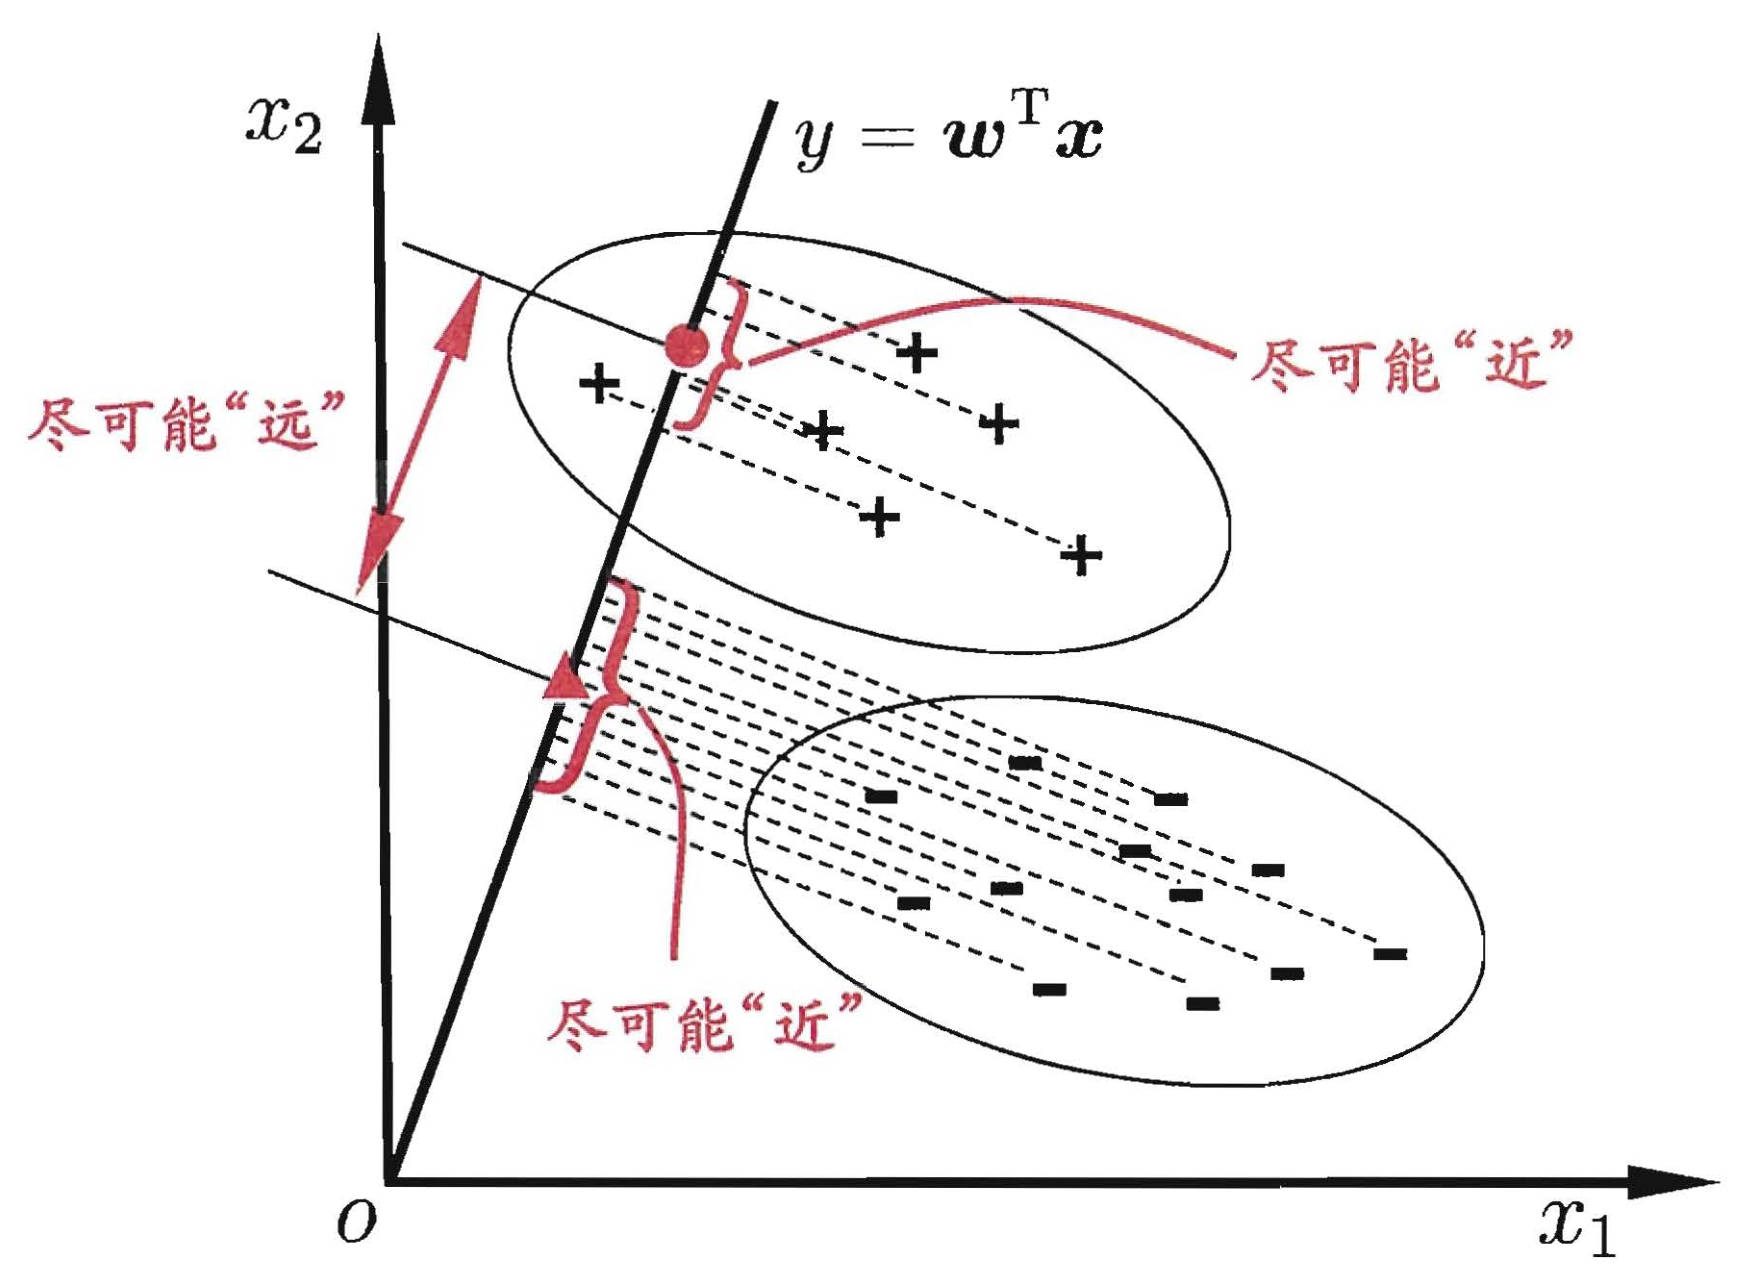
\includegraphics[width=0.5\linewidth]{textbook-fig3.3.jpg}
		      \caption{教材图 3.3}
		      \label{textbook_fig_3_3}
	      \end{figure}
	\item[(2)] \textbf{[5pts]} 请参考题干中的介绍与 (1) 中的现象, 简要回答:
	      \begin{itemize}
		      \item [(a)] 对照题干中LDA的优化目的, PCA的优化目的是什么?
		      \item [(b)] PCA相较于LDA有什么显著的不同点?
	      \end{itemize}
	\item[(3)] \textbf{[5pts]} \textit{下面, 我们先回顾教材第三章第四节中多分类 LDA 优化问题的矩阵形式. 考虑总类内散度是各个类别散度之和, 其矩阵形式为:
		      $\Sw = \sum_{i=1}^{N} {\Sw}_i.$
		      对于第 $i$ 个类别的类内散度矩阵定义如下:
		      ${\Sw}_i = \sum_{\x \in X_i} (\x - \muBold_i) (\x - \muBold_i)^\transposed.$
		      类似的, 总类间散度是各个类别中心相对于全局中心的散度之和, 其矩阵形式为:
		      $\Sb = \sum_{i=1}^{N} {\Sb}_i.$
		      对于第 $i$ 个类别的中心相对于全局中心的散度矩阵定义如下:
		      ${\Sb}_i = m_i (\muBold_i - \muBold) (\muBold_i - \muBold)^\transposed.$}\\
	      LDA事实上是在最小化\textbf{平均}类内散度和最大化\textbf{平均}类间散度, 其矩阵形式如 \eqref{lda-eigen} 所示. 其中, $d'$ 是降维后的维度, 严格小于数据维度 $d$.
	      \begin{equation}
		      \begin{aligned}
			      \max_{\W} \quad     & J(\W) = \frac{\tr{\W^\transposed \Sb \W}}{\tr{\W^\transposed \Sw \W}} = \frac{\tr{\W^\transposed \sbr{\sum_{i=1}^{N} {\Sb}_i} \W}}{\tr{\W^\transposed \sbr{\sum_{i=1}^{N} {\Sw}_i} \W}} = \frac{\frac{1}{N} \sum_{i=1}^{N} \tr{\W^\transposed {\Sb}_i \W}}{\frac{1}{N} \sum_{i=1}^{N} \tr{\W^\transposed {\Sw}_i \W}} \\
			      \mathrm{s.t.} \quad & \W^\transposed \W = \I_{d'}
		      \end{aligned}
		      \label{lda-eigen}
	      \end{equation}

	      \textbf{根据教材中的介绍, \eqref{lda-eigen} 可通过广义特征值分解进行求解.} 然而, 在某些现实场景下, 我们应用LDA的目的是提高分类准确率, 那么通常进一步希望\textbf{每个}类别散度尽可能小, \textbf{每个}类别中心相对于全局中心的散度尽可能大, \textbf{而非平均散度}. 因此, 考虑LDA的一种拓展形式:
	      \begin{equation}
		      \begin{aligned}
			      \max_{\W} \quad     & \sbr{\min_{i,j} J_{i,j}(\W)} = \frac{\min_{j} \{ \tr{\W^\transposed {\Sb}_j \W} \}}{\max_{i} \{ \tr{\W^\transposed {\Sw}_i \W} \}} \\
			      \mathrm{s.t.} \quad & \W^\transposed \W = \I_{d'}
		      \end{aligned}
		      \label{lda-pairwise}
	      \end{equation}
	      \textbf{请指出拓展形式 \eqref{lda-pairwise} 无法直接沿用原有形式 \eqref{lda-eigen} 的广义特征值求解算法的原因.} \\
	      提示: 指出求解时存在变量间的循环依赖关系.
	\item[(4)] \textbf{[5pts]} \textit{在线性代数中, 对于(半)正定矩阵 $\A, \B$, 若 $\sbr{\A-\B}$ 是正定矩阵, 则通常记作 $\A \succ \B$ 或 $\B \prec \A$; 若 $\sbr{\A-\B}$ 是半正定矩阵, 则通常记作 $\A \succcurlyeq \B$ 或 $\B \preccurlyeq \A$. 在优化问题中, 凸优化问题有多项式时间复杂度的理论保证, 能够高效求解. 凸优化问题的定义是: (i) 最小化的目标函数是凸函数, 或者最大化的目标函数是凹函数, 而且 (ii) 可行域是凸集合. 可行域是所有满足约束条件的控制变量取值 (又称可行解) 构成的集合.} \\
	      拓展形式 \eqref{lda-pairwise} 不能沿用原有形式 \eqref{lda-eigen} 的求解算法, 也不是凸优化问题. 为了高效求解, 需要探索一种将其转化成凸优化问题的方法. 已知原有形式 \eqref{lda-eigen} 可以松弛成如下凸优化问题:
	      \begin{equation}
		      \begin{aligned}
			      \max_{\W,r} \quad   & r                                             \\
			      \mathrm{s.t.} \quad & r \cdot \tr{\Sw \M} - \tr{\Sb \M} \leqslant 0 \\
			      \quad               & -r \leqslant 0                                \\
			      \quad               & \O \preccurlyeq \M \preccurlyeq \I_{d}       \\
			      \quad               & \tr{\M} = d'                                  \\
		      \end{aligned}
		      \label{lda-slack}
	      \end{equation}
	      请仿照原有形式 \eqref{lda-eigen} 的松弛形式 \eqref{lda-slack}, 给出拓展形式 \eqref{lda-pairwise} 的松弛形式, 并证明拓展形式的松弛形式是凸优化问题, 即同时满足条件 (i) 和条件 (ii).
	\item[(5)] \textbf{[5pts]} (\textit{本题为附加题, 得分计入卷面分数, 但本次作业总得分不超过 100 分}) 请证明:
	      \begin{itemize}
		      \item [(a)] 松弛形式 \eqref{lda-eigen} 和原有形式 \eqref{lda-slack} 的约束条件不等价;
		      \item [(b)] 当 $r \cdot \tr{\Sw \M} - \tr{\Sb \M} = 0$ 时, \eqref{lda-slack} 的可行域是 \eqref{lda-eigen} 可行域的凸包 (Convex Hull). 即: \eqref{lda-slack} 的可行解可以表示成 \eqref{lda-eigen} 的可行解的线性组合.
	      \end{itemize}
	      进而, \eqref{lda-slack} 的可行域是包含 \eqref{lda-eigen} 的可行域的最小凸集合, 即 \eqref{lda-slack} 对 \eqref{lda-eigen} 的放松程度是最小的, 因而能够使得凸问题 \eqref{lda-slack} 的解尽可能的接近原问题 \eqref{lda-eigen} 的解.
\end{enumerate}

\begin{solution}
此处用于写解答 (中英文均可)\\
(1)\begin{figure}[H]
  \centering
  \includegraphics[width=0.8\textwidth]{PCA.png}
  \caption{PCA的大致投影方向 }
  \label{fig:roc}
\end{figure}
(2)\\
(a)PCA的优化目的是:找到一个超平面,使得样本点在投影到这个超平面上后它们之间的投影能尽可能分开,即最大化投影后样本点的方差。\\
(b)显著不同点:\\
1.LDA 需要考虑类间的距离,也就是说 LDA 用到了样本点的标签,是一种监督学习的方法。但 PCA 并不需要用到样本点是属于哪一类的标签,是一种无监督学习的方法。\\
2.LDA 会选择分类性能最好的投影方向,而 PCA 会选择样本点投影具有最大方差的方向。\\
(3)按照原来 (4.1) 的形式,将其转化成下面的优化形式:
\[
\begin{aligned}
\min_{\W} & \quad \operatorname{-tr}(\W^T\S_{b}\W) \\\\\text{s.t. } & \quad - \operatorname{tr}(\W^T\S_{w}\W) = 1 
\end{aligned}
\]

写出其拉格朗日函数然后对 $\W$ 求导后可以通过广义特征值来求解,其形式如下:

\[
\S_{b}\W = \lambda \S_{w}\W
\]

注意到这里的形式相比教材里的形式还多了个 $\W^T\W = \I_{d'}$ 的约束,但实际上这个约束可以说是不起作用的,只起到了标准化模长的作用,因为 $(\S_{w})^{-1}\S_{b}$ 是一个实对称矩阵,那么其特征向量都是正交的,所以求得的 $\W$ 必然满足 $\W^T\W = \I_{d'}$,所以说这个约束实际上不起作用。\\
(4)问题 (4.2) 的松弛形式如下:

\[
\begin{aligned}
\max_{\W, r} & \quad r \\\text{s.t. } & \quad r \cdot w - b \leq 0 \\\\& \quad w \leq \operatorname{tr}(\S_{wi}\M) \\\\& \quad -b \leq \operatorname{tr}(\S_{bj}\M) \\\\& \quad -r \leq 0 \\\\& \quad \O \preceq \M \preceq \I_{d} \\\\& \quad \operatorname{tr}(\M) = d'
\end{aligned}
\]
证明:由于优化目标和优化函数都是仿射的,所以这个问题显然是凸优化问题。\\
 (5)\\
 (a) 要证明松弛形式 \eqref{lda-eigen} 和原有形式 \eqref{lda-slack} 的约束条件不等价,需要比较两个问题中的约束。

在 \eqref{lda-eigen} 中,约束是 $\W^\transposed \W = \I_{d'}$,这是一个关于 $\W$ 的正交约束,即要求 $\W$ 是一个正交矩阵。

而在 \eqref{lda-slack} 中,约束是 $r \cdot \tr{\Sw \M} - \tr{\Sb \M} \leqslant 0$,$-r \leqslant 0$,$O \preccurlyeq \M \preccurlyeq \I_{d'}$,以及 $\tr{\M} = d'$。这里引入了额外的变量 $r$ 和 $\M$,并且 $\M$ 被要求是一个介于零矩阵 $\O$ 和单位矩阵 $\I_{d'}$ 之间的半正定矩阵,且迹为 $d'$。

显然,\eqref{lda-eigen} 中的正交约束不能保证 \eqref{lda-slack} 中关于 $r$ 和 $\M$ 的所有约束都得到满足,反之亦然。因此,这两个问题的约束条件是不等价的。

(b) 当 $r \cdot \tr{\Sw \M} - \tr{\Sb \M} = 0$ 时,我们来考虑 \eqref{lda-slack} 的可行域与 \eqref{lda-eigen} 可行域的关系。

由于 $r \leqslant 0$,当 $r \cdot \tr{\Sw \M} - \tr{\Sb \M} = 0$ 时,实际上有 $r = 0$。在这种情况下,\eqref{lda-slack} 中的约束简化为 $\O \preccurlyeq \M \preccurlyeq \I_{d'}$ 和 $\tr{\M} = d'$。

此时,任何满足 $\W^\transposed \W = \I_{d'}$ 的 $\W$ 都可以扩展为一个满足 $\O \preccurlyeq \M \preccurlyeq \I_{d'}$ 和 $\tr{\M} = d'$ 的 $\M$,通过令 $\M = \W \W^\transposed$。这样的 $M$ 会自动满足 $\tr{\M} = d'$ 因为 $\tr{\W \W^\transposed} = \tr{\W^\transposed \W} = d'$。


因此,\eqref{lda-slack} 的可行解可以表示成 \eqref{lda-eigen} 的可行解的线性组合,即 \eqref{lda-slack} 的可行域是 \eqref{lda-eigen} 可行域的凸包。

综上所述,\eqref{lda-slack} 的可行域是包含 \eqref{lda-eigen} 的可行域的最小凸集合,这意味着 \eqref{lda-slack} 对 \eqref{lda-eigen} 的放松程度是最小的,从而使得凸问题 \eqref{lda-slack} 的解尽可能接近原问题 \eqref{lda-eigen} 的解。
\end{solution}

\newpage

\section{[25pts] 编程实验: LDA 与多分类}

\begin{tcolorbox}
	\textbf{[注意事项]} 请不要修改或提交 \texttt{utils.py}; 在合理范围内, 运行时间和错误率不作为评分依据. 实现过程中只允许使用 NumPy 和 SciPy 提供的矩阵运算接口, 否则相应题目不计入分数.

	此外, 对于题 (3,4,5), 如果调用 Sci-Kit Learn 实现二分类模型, 基于二分类模型实现多分类模型, 并且画出相应图像, 可计入题 (4,5) 得分, 但不计入题 (3) 得分.

	\textbf{[符号约定]} \texttt{x} 是形状为 \texttt{(m, d)} 的矩阵, 其元素为32位浮点数; 在题 (1,3,4,5) 中, \texttt{y} 是形状为 \texttt{(m,)} 的向量, 其元素为32位整数; 在题 (2) 中, \texttt{y} 是形状为 \texttt{(m, 2)} 的向量, 其元素为32位浮点数. 其中: \texttt{m} 为样例个数, \texttt{d} 为样例维度; 标签从 \texttt{0} 开始, 例如共20类时, 标签依次是 $\{\mathtt{0}, \cdots, \mathtt{19}\}$.
\end{tcolorbox}

\begin{enumerate}
	\item[(1)] \textbf{[5pts]} 根据 \texttt{main.py} 中的框架代码, 实现LDA降维, 通过 \texttt{lda\_sanity\_check} 测试, 并在 \texttt{HW2.pdf} 中展示运行后的终端输出截图.
	\item[(2)] \textbf{[5pts]} 基于 (1) 分别把训练数据和测试数据降至两维, 并绘制在同一张散点图上, 在 \texttt{HW2.pdf} 中展示. 注意: 同类别的点应当使用同一颜色, 不同类别的数据点应当使用不同颜色.
	\item[(3)] \textbf{[5pts]} 分类任务可以被归结为一种特殊的回归任务, 可参考 \texttt{sklearn} 中的内容: \href{https://scikit-learn.org/stable/modules/linear_model.html#classification}{[Link]}. 对于二分类任务, 我们任选一类作为正类, 另一类成为负类. 对于正类样本 $\x_+$, 约定 $y_+ = 1$, 对于负类样本 $\x_-$, 约定 $y_- = -1$, 对于训练得到的分类器 $f$ 和测试样例 $\x$, 如果 $f(\x) \geqslant 0$ 预测为正类, 否则预测为负类. \\根据框架代码, 按照上述约定实现基于岭回归的二分类模型, 通过\\ \texttt{classifier\_2\_sanity\_check} 测试, 并在 \texttt{HW2.pdf} 中展示运行后的终端输出截图.
	\item[(4)] \textbf{[5pts]} 基于 (3) 中的二分类模型, 通过 OvR 策略将其拓展为多分类模型, 通过\\ \texttt{classifier\_n\_sanity\_check} 测试, 最后在 \texttt{HW2.pdf} 中展示运行后的终端输出截图.\\提示: 判断测试样例的预测结果时, 可以依照教材实现, 即若有多个分类器预测为正类或者没有分类器预测为正类, 则考虑各分类器的预测置信度 ($f(\x)$ 之值), 选择置信度最大的类别标记作为分类结果.
	\item[(5)] \textbf{[5pts]} 基于 (4) 绘制并在 \texttt{HW2.pdf} 中展示\textbf{训练错误率和测试错误率随 $\lambda$ 变化的折线图}. 注意: 图像横轴为 $\lambda$; 训练错误率和测试错误率应当使用不同颜色的曲线.
\end{enumerate}

\begin{solution}
	此处用于写解答 (中英文均可)\\
 (1)
  \begin{figure}[H]
    \centering
    \includegraphics[width=0.8\textwidth]{LDAcheck.png}\\
    \caption{LDAcheck}
    \label{fig:roc}
\end{figure}
 (2)
 \begin{figure}[H]
    \centering
    \includegraphics[width=0.8\textwidth]{LDA.png}\\
    \caption{LDA}
    \label{fig:roc}
\end{figure}
(3)(4)
 \begin{figure}[H]
    \centering
    \includegraphics[width=0.8\textwidth]{classifierCheck.png}\\
    \caption{classifierCheck}
    \label{fig:roc}
\end{figure}
(5)
 \begin{figure}[H]
    \centering
    \includegraphics[width=0.8\textwidth]{折线图.png}\\
    \caption{训练错误率和测试错误率随$\lambda$变化的折线图}
    \label{fig:roc}
\end{figure}
\end{solution}

\newpage

\section*{Acknowledgments}
允许与其他同样未完成作业的同学讨论作业的内容, 但需在此注明并加以致谢; 如在作业过程中, 参考了互联网上的资料或大语言模型的生成结果, 且对完成作业有帮助的, 亦需注明并致谢.

\end{document}
